\section{Experiment P2F: conditional accuracy--communication consolidation}
\label{sec:p2f}
\subsection{Purpose and evidence accounting}
P2F consolidates P2A--P2E without running new simulations or changing the estimator. Its purpose is to identify useful tested communication budgets, distinguish relative geometry from absolute localization, and state which conclusions survive sensor and range degradation. The four moving nodes, fixed trajectories, known initial poses, 60 s duration, and 20 matched seeds remain the scope of the evidence.

The input contains 1960 source run records. Repeated endpoints are not independent replications: 200 endpoint checks agree numerically, leaving 1760 distinct seed records for 88 designs. P2A's zero/full endpoints audit P2B; the clean P2D and reference P2E endpoints audit earlier designs. The consolidated catalogue retains source provenance and SHA-256 hashes. Every design contains exactly the same 20 seed identifiers. Attempted, received, and accepted counts satisfy their ordering constraints, and the per-seed squared fleet error decomposition into centroid and relative-shape error is checked.

\subsection{Cost, conditional frontiers, and uncertainty}
Communication cost is the number of \emph{attempted undirected UWB exchanges} over 60 s, including failures and rejected observations. The full reference attempts 3600 exchanges; normalized cost is the attempted count divided by 3600. This is a transaction-count proxy, not measured radio energy or a count of protocol packets.

For each fixed sensor condition, process-covariance treatment, range condition, and update rule, a design is empirically nondominated if no tested design has no greater attempted cost and no greater error, with at least one strict improvement. P2F calculates separate frontiers for mean shape, mean fleet, mean worst-node, and empirical 95th-percentile shape RMSE. Exact ties remain nondominated; a numerical tolerance of \(10^{-12}\) only guards arithmetic precision. These are frontiers of tested designs, not estimates of a continuous optimum.

Schedule and timing remain labelled. P2C's cyclic, random, geometry, and information choices share per-tick opportunities and therefore isolate pair selection. P2B's simultaneous all-link rounds use different timing. Their inclusion in a whole-design frontier is valid, but their differences cannot be attributed solely to pair choice. P2D has only 360 attempted exchanges: each reliability condition is a single-budget slice, not a reliability frontier curve.

Seed variability uses sample standard deviation. Empirical percentiles use the 20 seed RMSE values and linear interpolation; a percentile of seed-level trajectory RMSE is not a percentile of instantaneous error. Paired differences use the same seeds, with 30000 bootstrap resamples and a fixed analysis RNG seed. Their 95\% intervals are descriptive, unadjusted for multiple comparisons, and do not account for path or scenario uncertainty. Mean and percentile target crossings are reported separately from the observed number of passing seeds.

\subsection{Clean reference: a useful shape frontier and an absolute-error floor}
Figure~\ref{fig:p2f_clean} shows all tested positive-budget designs under the reference IMU, frozen process covariance, clean ranges, and ordinary update. Zero-UWB remains in the numerical catalogue but is omitted from logarithmic plots: its mean shape, fleet, and worst-node RMSE are 2.0273, 2.3222, and 3.2375 m. The mean-shape frontier selects geometry at 180 attempts (0.1066 m), information at 360 (0.0789 m), uniform all-link rounds at 720 (0.0670 m) and 1800 (0.0543 m), and all pairs at 3600 (0.0456 m). These labels change with the objective; the worst-node frontier differs from the shape frontier.

\begin{figure}[htbp]
\centering
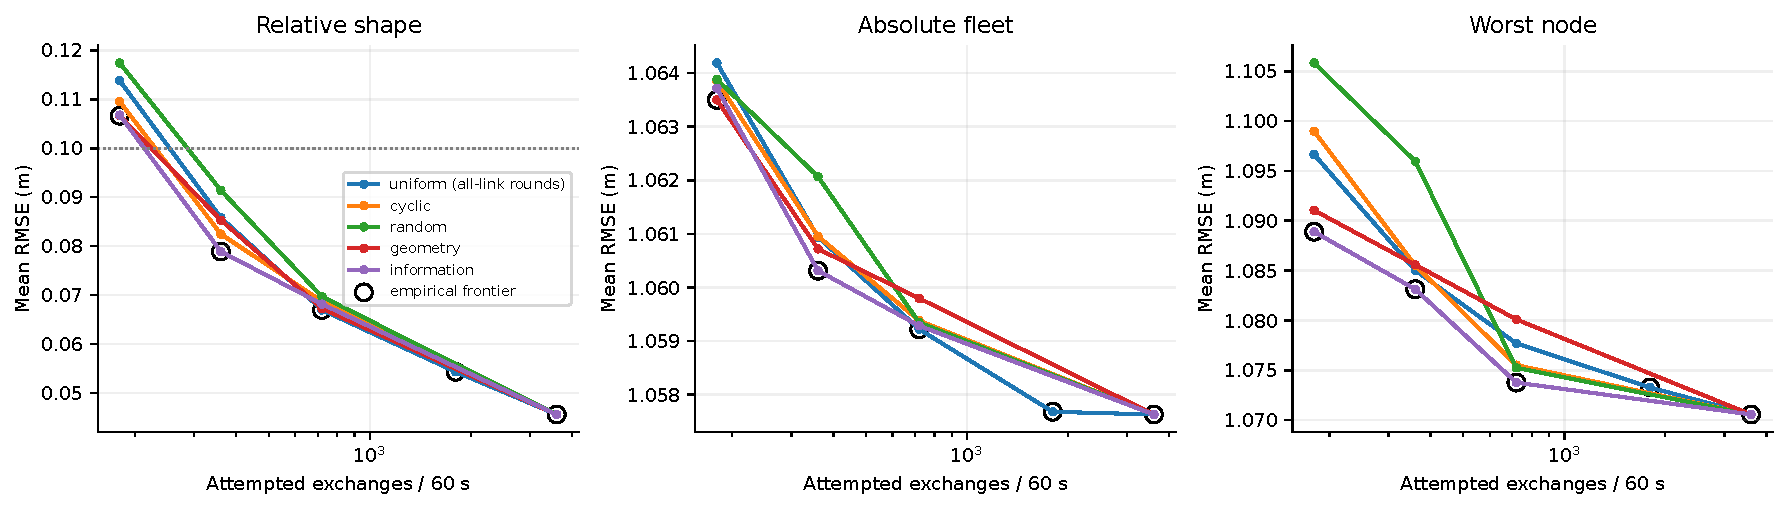
\includegraphics[width=\textwidth]{figures/phase2/p2f_clean_frontiers.pdf}
\caption{P2F clean-reference means over 20 seeds. Black rings mark empirical nondominated designs separately for each objective. Positive attempted budgets use a logarithmic axis; the zero-budget endpoint is retained in the catalogue. Uniform all-link rounds differ in timing from P2C pair-selection designs. Connecting segments guide the eye and do not imply tested intermediate budgets.}
\label{fig:p2f_clean}
\end{figure}

Empirical selection of a lowest mean does not establish a robust scheduling advantage. At 360 attempts, information minus cyclic has mean shape difference \(-0.00356\) m, improves 13/20 seeds, and its paired bootstrap interval includes zero. Differences are only millimetres in this clean four-node setting. Retain cyclic as the transparent practical baseline; report the selected frontier as a descriptive comparison rather than a recommendation to switch policies.

The cyclic mean shape error falls from 0.1095 m at 180 attempts to 0.0824 m at 360 and 0.0687 m at 720, reaching 0.0456 m at full communication. Meanwhile full-rate absolute fleet RMSE remains about 1.058 m and centroid RMSE about 1.056 m. Pairwise ranges improve relative geometry but provide no continuing global position observation to constrain common translation drift. More pairwise communication alone does not resolve this limitation.

\subsection{Target decisions depend on the condition}
Table~\ref{tab:p2f_targets} uses the predefined descriptive 0.10 m shape target. Entries are the smallest \emph{tested} budget meeting the indicated statistic. The cyclic reference scope includes its zero/full endpoints; the ordinary uniform scope includes the P2B rate sweep. No intermediate budget is inferred. A dash means the target was not reached at any tested budget, including 3600.

\begin{table}[htbp]
\centering\small
\begin{tabular}{lrrr}
\toprule
Clean condition and design family & Mean target & p95 target & Passing seeds$^*$\\
\midrule
Reference, cyclic, frozen Q & 360 & 720 & 18/20\\
Reference, uniform rounds, frozen Q & 360 & 720 & 15/20\\
Half white noise, cyclic, frozen Q & 360 & 360 & 19/20\\
Half white noise, cyclic, rescaled Q & 180 & 360 & 11/20\\
Half bias drift, cyclic, frozen Q & 360 & 360 & 19/20\\
Fourfold white noise, cyclic, either Q & --- & --- & ---\\
Tenfold bias drift, cyclic, frozen Q & --- & --- & ---\\
Both degraded, cyclic, either Q & --- & --- & ---\\
\bottomrule
\end{tabular}
\caption{Smallest tested attempted-exchange budget meeting the mean or empirical p95 shape target. $^*$Passing seeds are evaluated at the mean-target budget. ``Either Q'' denotes the frozen and white-noise-rescaled treatments tested in P2E, not arbitrary covariance tuning.}
\label{tab:p2f_targets}
\end{table}

Across all clean-reference designs, the mean-target selection is information at 360 and the p95-target selection is random at 720. Their within-budget rankings do not alter the reference's tested budget requirements, and selection among many empirical means or percentiles can be optimistic. Report design-specific results rather than inferring superiority from these rankings.

\begin{figure}[htbp]
\centering
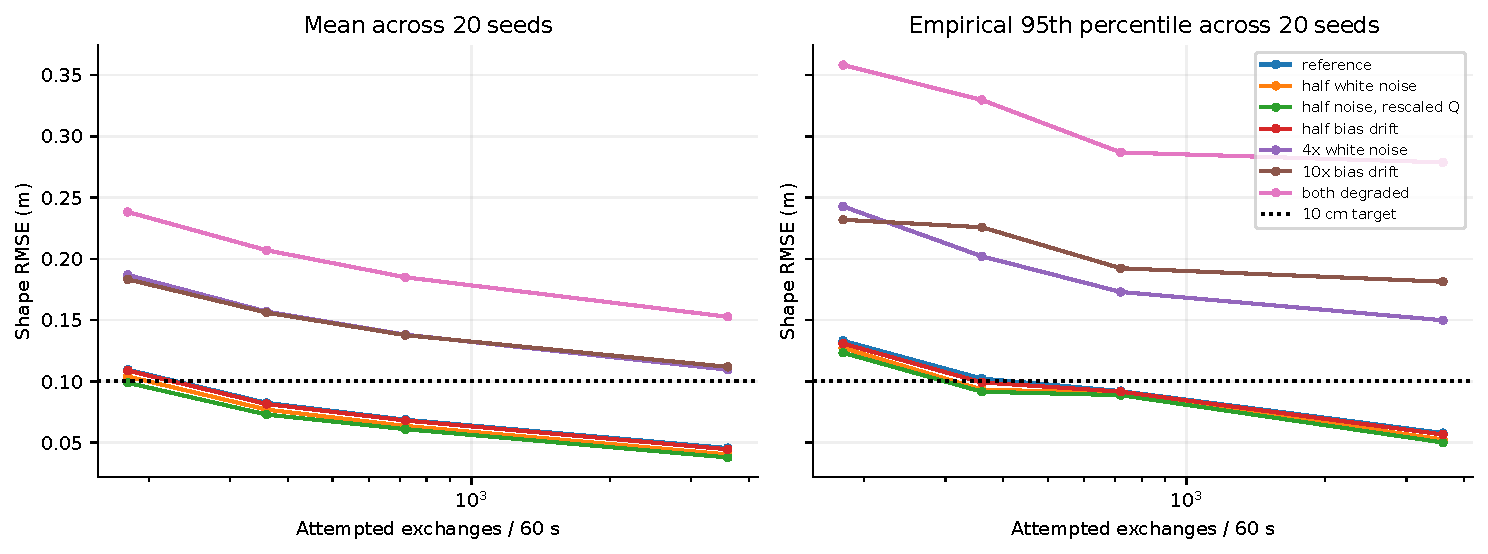
\includegraphics[width=\textwidth]{figures/phase2/p2f_sensor_targets.pdf}
\caption{Conditional cyclic shape curves and their empirical p95 values; full communication uses all pairs. Q rescaling is displayed explicitly for the lower-noise example. The complete decision catalogue also retains the rescaled high-noise cases, which fail the target. Lines connect tested positive budgets only.}
\label{fig:p2f_sensor}
\end{figure}

Lower noise with rescaled Q meets the mean target at 180 attempts, but only 11/20 seeds pass and p95 is 0.1234 m. Its p95 criterion still needs 360. This crossing does not establish a reliable 50\% communication saving. Conversely the degraded sensors retain mean shape errors of 0.1096, 0.1119, and 0.1527 m at full communication. A budget choice must therefore specify its sensor and covariance assumptions. White-noise rescaling is not a bias-state model, and these amplitude changes are not calibrated commercial IMU grades.

\subsection{Reliability can matter more than pair selection}
Figure~\ref{fig:p2f_reliability} retains the single-budget nature of P2D. With cyclic ordinary updates, 30\% loss meets the mean shape target (0.0919 m), whereas 50\% loss does not (0.1100 m). Outliers raise mean error to 0.2955 m; gating restores 0.0838 m, an effect much larger than the clean pair-selection differences. Persistent biased ranges remain harder: gated cyclic has mean 0.0956 m, but gated information has 0.1305 m. None of the reliability cases, including clean gated, meets the empirical p95 target at this budget. The clean ordinary reference also fails that criterion at 360.

\begin{figure}[htbp]
\centering
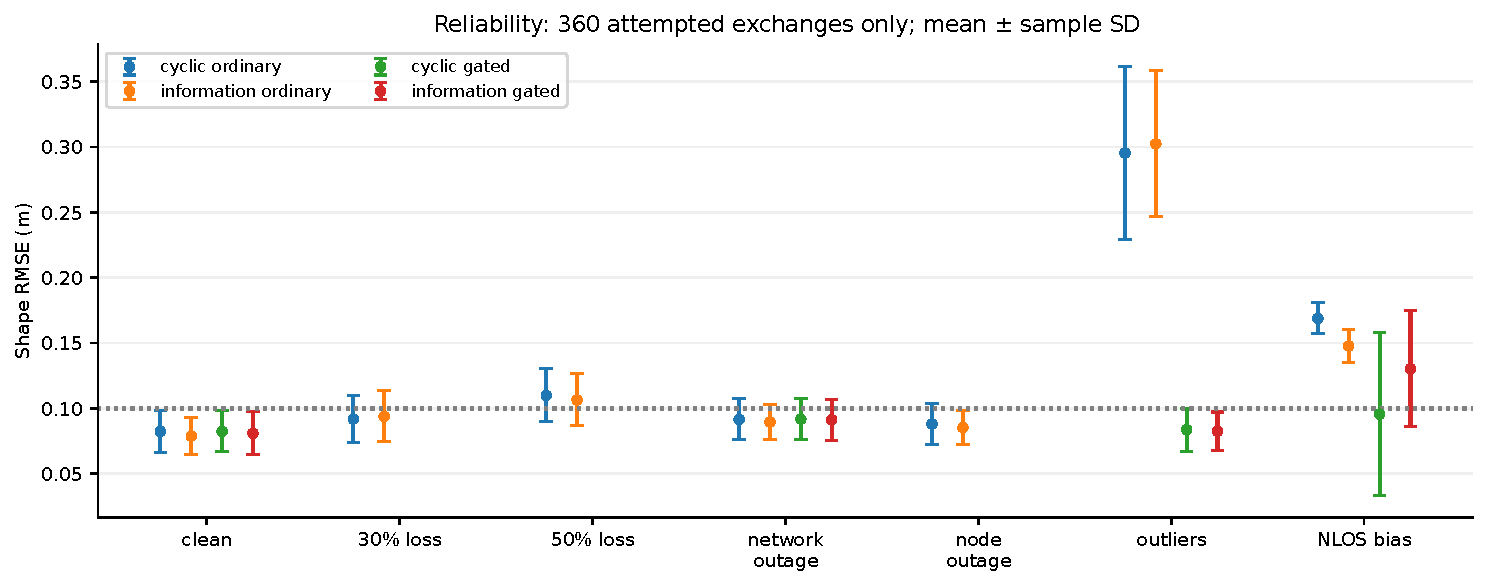
\includegraphics[width=\textwidth]{figures/phase2/p2f_reliability_slice.pdf}
\caption{Reliability evidence at 360 attempted exchanges only. Bars indicate one sample standard deviation over seeds, not confidence intervals. Missing gated entries were not tested. Cyclic and information schedules have matched timing; the complete catalogue separately retains the differently timed uniform reference.}
\label{fig:p2f_reliability}
\end{figure}

Information selection under persistent bias reverses its ordinary-update advantage after gating: the gated paired shape difference is +0.03484 m, with descriptive 95\% interval [0.01997, 0.04804] m. Rejected information leaves predicted uncertainty high, encouraging repeated attempts on the problematic pair. Therefore a clean covariance score cannot be assumed to remain useful under rejection or missing data. Received and accepted counts describe these mechanisms but do not replace attempted cost. Passing the mean at 360 does not identify a minimum reliability budget; no other budget was tested under those stresses.

\subsection{Decision and reproducibility}
For this benchmark, cyclic at 360 attempts is a useful clean mean-target operating point, using 10\% of full attempted communication; 720 attempts, or 20\%, meets the empirical p95 criterion. These are tested choices for this scenario, not deployment guarantees. The principal practical gains are reducing redundant clean ranging and protecting updates from isolated corruptions. Specialized information selection has no consistent clean shape advantage, and persistent bias can invalidate its benefit. Absolute error remains dominated by common drift.

The next planned extension is P2G: add a continuing global position reference to one existing moving node and compare the same three non-reference nodes at matched UWB budgets and sensor realizations. Start with an ideal reference to bound its value; noisy and intermittent reference cases must propagate uncertainty and count reference updates separately. Reliability-aware selection and a bias-state estimator remain separate future experiments.

The configuration is \texttt{configs/phase2f.yaml}. Run these Python scripts in order to regenerate numerical outputs and figures:
\begin{quote}\footnotesize
\url{experiments/analyze_phase2f.py}\\
\url{experiments/generate_phase2f_figures.py}
\end{quote}
The seed catalogue, design summaries, target decisions, paired comparisons, endpoint audit, and source hashes are stored under \texttt{results/phase2/p2f/}. The compact CSVs preserve the evidence required to reproduce consolidation without rerunning simulations.
